\subsection{Architettura di dettaglio: strategy}
\begin{figure}[hb]
	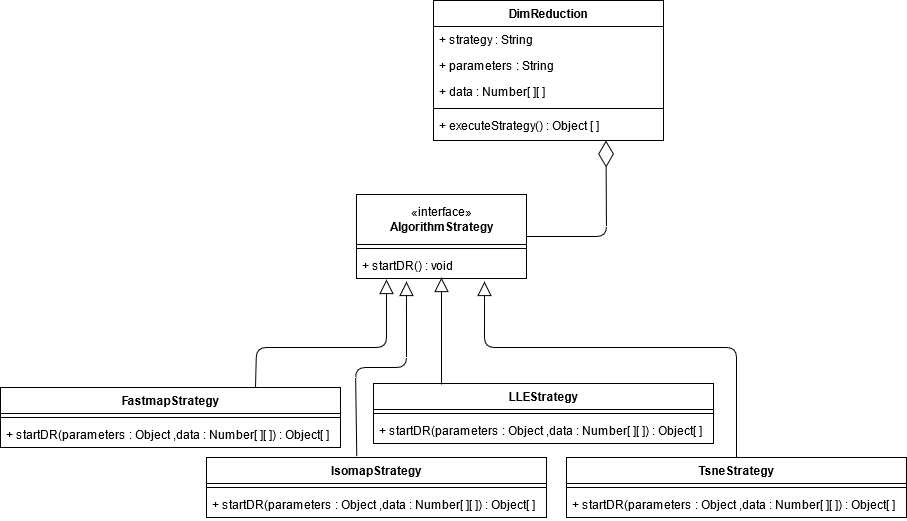
\includegraphics[width=15.8cm]{Images/StrategyPattern}
	\centering
	\caption{Strategy pattern per la scelta dell'algoritmo di riduzione dimensionale}
\end{figure}
Lo \glo{Strategy pattern} è stato adottato per modellare la scelta dell'algoritmo di riduzione dimensionale. Il pattern si compone di un solo metodo: \texttt{startDR()} che effettua la riduzione dimensionale dei dati inseriti. Questo metodo è implementato diversamente, in base alle necessità dell'algoritmo. Come ci si aspetta, lo Strategy è istanziato solamente una volta da \texttt{DimReduction} dopo che l'utente ha scelto l'algoritmo.